\documentclass[12pt]{article}
\usepackage{amsmath}
\usepackage{csvsimple}
\usepackage{graphicx}
\graphicspath{ {./../images/} }
\usepackage{hyperref}
\usepackage[latin1]{inputenc}
\usepackage{listings}

\DeclareMathOperator{\Tr}{Tr}

\lstset{
  columns=fullflexible,
  breaklines=true,
  }

\twocolumn

\title{Local Assortativity on Networks with Unbalanced Classes}
\author{Rebecca Cohen}

\begin{document}
\maketitle
\section{Introduction}
Assortativity and its limitations

Multiscale mixing -- include PPR and TotalRank

Peel et. al find considerable variation in $r_\ell$ on both random and empirical networks.  However, it is not obvious whether local differences in assortativity are the result of differences in the probability of nodes forming in-group vs. out-group edges, or whether there may be other factors that influence the distribution of $r(\ell)$.

This paper will analyze the distribution of $r(\ell)$ with respect to class size.  We find that otherwise comparable nodes in larger classes tend to have higher $r(\ell)$ scores on both assortative and disassortative networks.  We develop a theoretical prediction of $r(\ell)$ based on a DC-SBM null model and use numerical experiments to validate its predictions.

\section{Methods}
To test the influence of class size on local assortativity, we use null models in which there is no fine-grained assortative structure and record how $r_\ell$ varies relative to class size.  This experimental setup considers two different null models, the Erdos-Renyi random graph, which has no assortatitive structure, and a simple stochastic block model (SBM) with equal in- and out-group pairing probabilities for all classes of nodes.  The Erdos-Renyi random graph 

\section{Multiscale Mixing In Unbalanced Classes}
Include simulations and real data


\section{Blockwise Expectation of Multiscale Mixing Scores Under DC-SBM}
The multiscale mixing score $r(\ell)$ is defined
\begin{equation}
  r(\ell) = \frac{1}{Q_{max}} \sum_g (e_{gg}(\ell) - a_g^2)
\end{equation}

where 
\begin{equation}
  e_{gg}(\ell) = \sum_i \sum_j w_{\text{multi}}(i; \ell) \frac{A_{ij}}{k_i} \delta(z_i, z_j) 
\end{equation}

and $k_i$ is the degree of the ith node, while $w_{\text{multi}}(i; \ell)$ is the $i$th element of the totalRank vector centered at node $\ell$.  With two key assumptions, we can calculate the expectation of $r(\ell)$ under a degree-corrected stochastic block model (DC-SBM).  While neither is assumption is true in general, numerical simulations support the predictions resulting from this calculation:

\begin{enumerate}
  \item The degree of every node is equal to its expected degree ($k_i = \theta_i$)
  \item The network is fully connected
\end{enumerate}

Assumption 1 allows us to treat node degrees and edge counts as constants.  Without this assumption, both $e_gg(\ell)$ and $a_g$ are the ratios of two Poisson random variables, and it is theoretically possible for the denominator to equal 0, rendering the expectations of these measures undefined.  However, on networks large enough to be interesting, the edge count is extremely unlikely to be zero, and tends to be close to its expectation under the DC-SBM.  More work is needed to develop probabilistic bounds on the error, but numerical simulations support the utility of this naive appoximation (see figure BLAH).    

Assumption 2 will become necessary when we compute transition probabilities for the blockwise personalized pageRank. 

ALTERNATE FRAMING: random rewiring of an empirical network.

TODO: Define the DC-SBM parameters

Under this simplified regime, since every node has its expected degree,
\begin{equation}
  a_g = \sum_i \sum_j A_{ij} \delta(z_i, g) = \sum_h \mathcal{M}_{gh}
\end{equation}

Noteably, $a_g$ is a constant here so 
\begin{equation}
  \langle r(\ell) \rangle = \frac{\langle e_{gg}(\ell) \rangle - \sum_g \big( \mathcal{M}_{gh} \big)}{1 - \sum_g \big( \mathcal{M}_{gh} \big)}
\end{equation}

To compute the expectation of $e_{gg}(\ell)$, we build on recent work by Chen et al \cite{chen:2020} showing that
\begin{equation}
  \langle w_\alpha (i ; \ell) \rangle = \theta_i w_\alpha(g)
\end{equation}
where $w_\alpha(i;\ell)$ is the personalized pageRank of node $i$ with respect to node $\ell$ given a fixed $\alpha$, and $w_\alpha$ is the blockwise personalized pageRank.
TODO: blockwise PPR! 

Using the linearity of both expectation and integration, we find the TotalRank \cite{boldi:2005} \cite{Peel:2018} of node $i$ with respect to $\ell$:
\begin{equation}
  \langle w_\text{multi} (i ; \ell) \rangle = \theta_i \int_0^1 w_\alpha(g) d\alpha
\end{equation}

Since $w_\alpha (g;\ell)$ can be computed in just $O(C^2)$, this integral can easily be approximated numerically from the results for many choices of $\alpha$.

Under assumption 1, $k_i = \theta_i$ for every node, so $k_i$ and $\theta_i$ will cancel in the equation for $\langle e_{gg} (\ell)$, so
\begin{equation}
    \langle e_{gg}(\ell) \rangle = \big \langle \sum_i \sum_j w_\text{multi}(z_i; \ell) A_{ij} \delta(z_i, z_j) \big \rangle\\
\end{equation}

In theory, $w_\text{multi}$ is not independent of $\sum_i \sum_j A_{ij} \delta(z_i, z_j)$, as the existance or nonexistance of each in-group edge has a impact on the blockwise transition matrix.  However, with a sufficiently high mean degree, the results will be close to independent, so we approximate
\begin{equation}
  \begin{aligned}
    \langle e_{gg}(\ell) \rangle &= \big \langle w_\text{multi}(g; \ell) \big \rangle \big \langle \sum_i \sum_j A_{ij} \delta(z_i, z_j) \big \rangle \\
    &= w_\text{multi}(g; \ell) \mathcal{M}_{gg}
  \end{aligned}
\end{equation}

Substituting the expection of $\langle e_{gg}(\ell)\rangle$ back into equation NUMBER, we find

\begin{equation}
  \langle r(\ell) \rangle = \frac{\mathcal{M}_{gg} w_\text{multi}(g; \ell) - \sum_g \big( \mathcal{M}_{gh} \big)}{1 - \sum_g \big( \mathcal{M}_{gh} \big)}
\end{equation}

Equation NUMBER depends only on the mixing matrix and blockwise PPR vector.  This means that $\langle r(\ell) \rangle$ will be the same for every element of each block, regardless of its degree.  It also means that we can compute $\langle r(\ell) \rangle$ directly from the mixing matrix.

\section{Numerical Experiments}
The calculation above relied on some highly unrealistic but conveninent assumptions about the DC-SBM.  To test how well these predictions work in practice, we generate networks using a DC-SBM and compare the distribution $r_\ell$ scores with the theoretical prediction from equation NUMBER.

For these experiments, we select a heterogeneous distribution of block sizes and degree distributions.  We keep the ratios of block sizes roughly fixed between trials, with adjustments to account for rounding.  We generate both assortative and disassortative networks, keeping in-group and out-group probability of an edge existing constant between classes, so the only structural difference between different classes is the size of the class. 

\begin{figure}[h!]
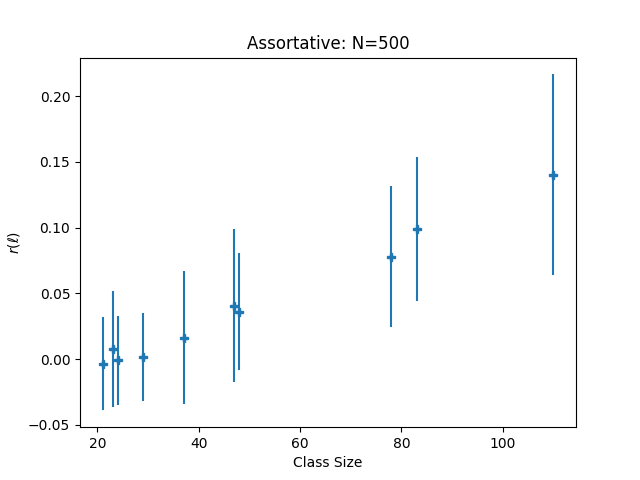
\includegraphics[width=0.5\textwidth]{assortative_N_500.png}
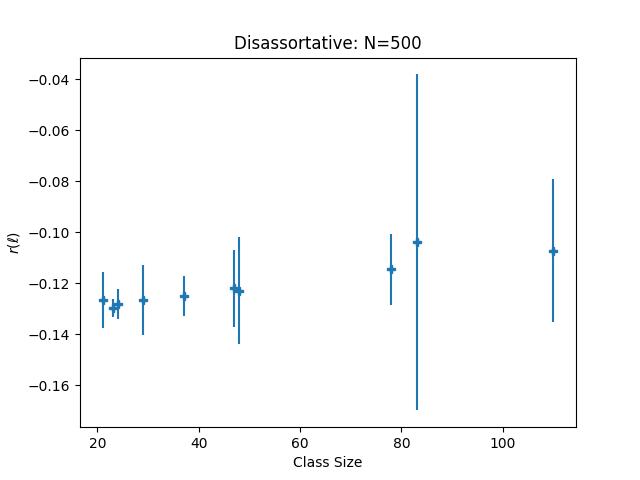
\includegraphics[width=0.5\textwidth]{disassortative_N_500.png}
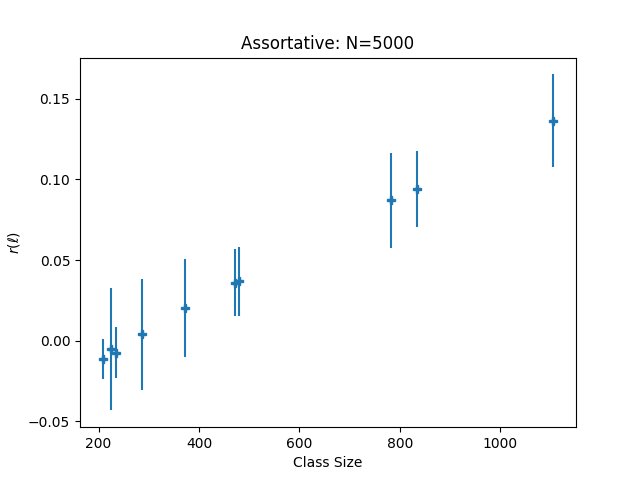
\includegraphics[width=0.5\textwidth]{assortative_N_5000.png}
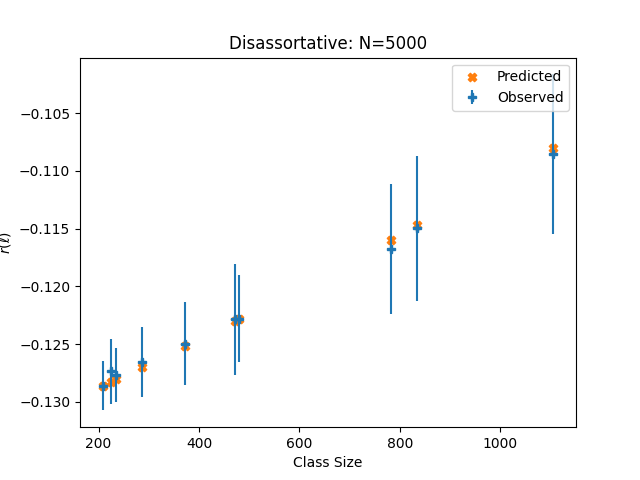
\includegraphics[width=0.5\textwidth]{disassortative_N_5000.png}
\caption{Distribution of $r(\ell)$ on DC-SBM random networks with uneven class sizes and heavy-tailed degree distribution.  Networks are constructed to have similar proportions within each class and similar in- and out-group pairing probabilities.  Errorbars show the standard deviation within each class}
\end{figure}

Figure NUMBER shows the distribution of $r_\ell$ within each class on a single DC-SBM for both assortatiive and disassortatiive nettworks.  Mean scores appear close to the theoretical prediction and the standard deviation decreases as the size of the network grows.  These networks were constructed in such a way that larger networks had higher mean degree, which decreases the impact of random fluctuations due to a small number of edges.  

\begin{figure}[h!]
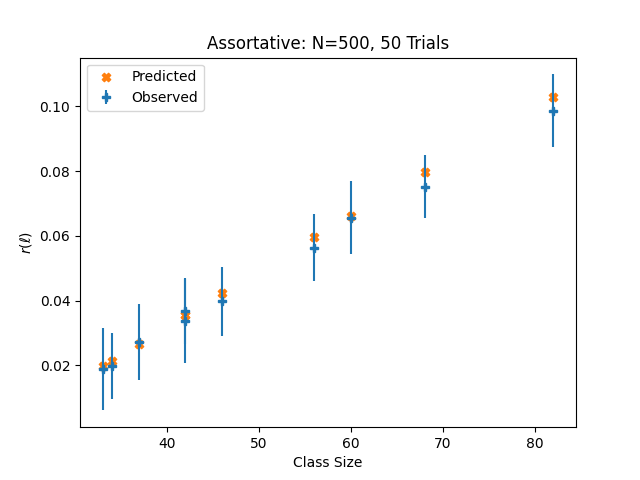
\includegraphics[width=0.5\textwidth]{assortative_N_500_trials_50.png}
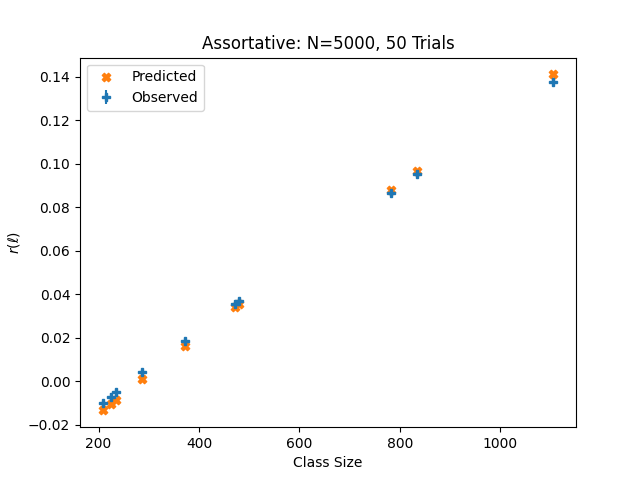
\includegraphics[width=0.5\textwidth]{assortative_N_5000_trials_50.png}
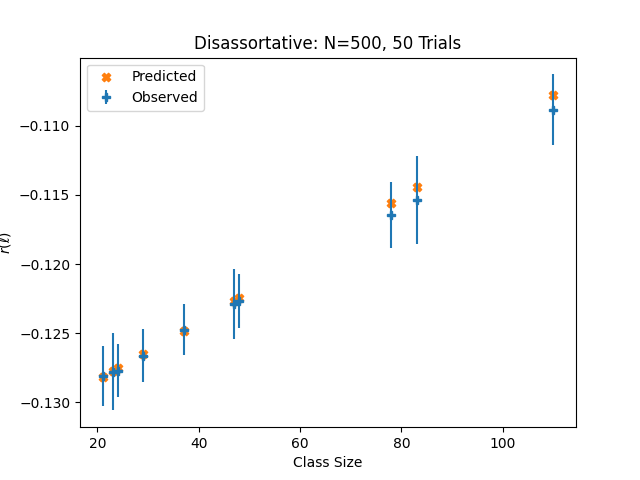
\includegraphics[width=0.5\textwidth]{disassortative_N_500_trials_50.png}
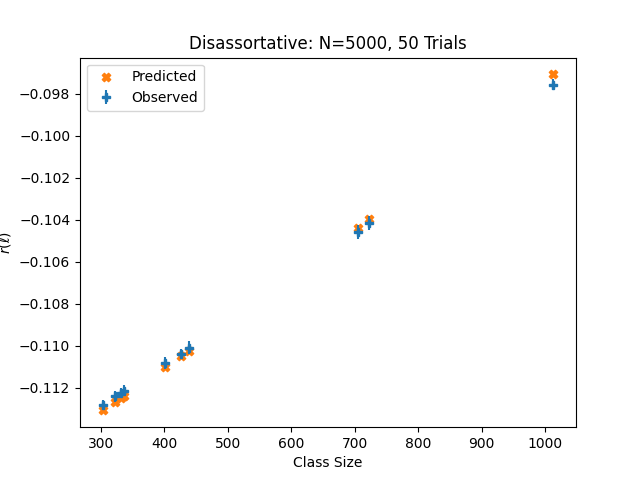
\includegraphics[width=0.5\textwidth]{disassortative_N_5000_trials_50.png}
\caption{Classwise mean $r(\ell)$ across 50 trials on DC-SBM random networks with identical parameters}
\end{figure}

In figure NUMBER we consider the same unbalanced partition of classes, but compare the classwise mean of $r(\ell)$ scores across 50 different random networks generated from the same parameters.  Once again, $r(\ell)$ values appear to be centered around the theoretical prediction, and variance decreases as $n$ grows.  At $N=1000$ we begin to see the magnitude of the error in our theoretical analysis as the observed distribution converges.  It appears that the theoretical prediction slight underestimates $r(\ell)$ on small classes and overestimates it on large classes, for both assortative and disassortative and disassortative networks.

\begin{figure}[h!]
\includegraphics[width=0.5\textwidth]{assortative_N_500block_9.png}
\includegraphics[width=0.5\textwidth]{assortative_N_5000block_9.png}
\includegraphics[width=0.5\textwidth]{disassortative_N_500block_9.png}
\includegraphics[width=0.5\textwidth]{disassortative_N_5000block_9.png}
\caption{Distribution of $r(\ell)$ within one block of DC-SBM}
\end{figure}

In figure NUMBER we take a closer look at the distribution of $r_\ell$ within a single class of a single random network.  The distribution appears to be centered around the theoretical prediction.  It is unimodal, fairly symmetric and not very heavy-tailed, appearing similar in shape to a Poisson distribution.

\section{Discussion}

\bibliographystyle{plain} % We choose the "plain" reference style
\bibliography{refs} % Entries are in the refs.bib file

\section*{Code}

\end{document}